\chapter{Design}
\label{cha:Design}
For the initial development of the simulator I focused on creating a working prototype for S2S merges. The S2S merge is one of the most simple merge scenarios that an autonomous vehicle might encounter. The designs here can then be expanded at a later date to include some of the other scenarios in \ref{sec:Merge Types}.

\section{Map}
\label{sec:Map}
In order to build the map using the user's parameters we will need to calculate the relative positions of the lane entrances and exits as well as the locations of the data collection lines and spawn points. A more detailed analysis of the mathematics used to calculate these positions can be found in Appendix \ref{sec:S2SMapCalculations}.

\subsection{Target Lane Coordinates}
\label{subsec:Target Lane Coordinates}
The target lane entrance will have a Y-coordinate equal to half of the lane width. In fact, every coordinate that target vehicles travel on will have a Y-coordinate equal to half the lane width. The entrance's X-coordinate will depend on whether the target lane, plus the merge zone length, is longer than the base width of the merging lane, that is, the horizontal distance the merging lane covers. You can see this distance indicated in Figure \ref{fig:baseWidth}.

\begin{figure}[htb]
\centering
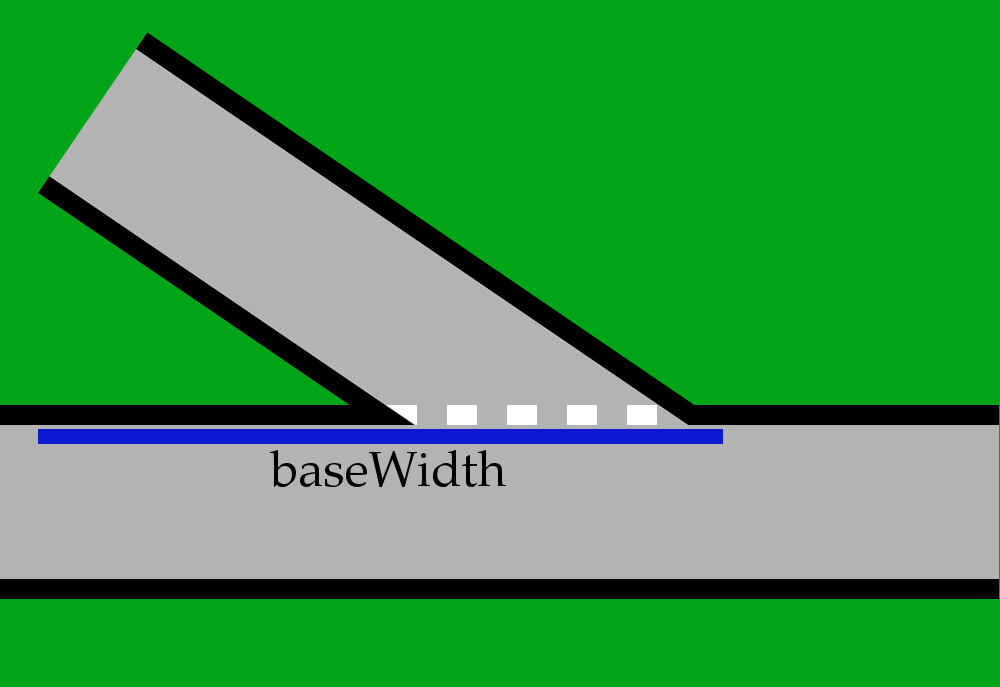
\includegraphics[width=8cm]{designNotes/baseWidth.png}
\caption{A diagram indicating the base width of the merging lane.}
\label{fig:baseWidth}
\end{figure}

If the target lane is longer then the entrance X-coordinate will be $0$. If not then we have to do further calculations. The total width of the simulation is given by equation \ref{targetLongerWidth} if the target lane has $x=0$ and equation \ref{mergeLongerWidth} if not.

\begin{equation} \label{targetLongerWidth}
	\begin{split}
		width = & targetLeadInDistance \\
			    & + mergeZoneWidth \\
			    & +	targetLeadOutDistance
	\end{split}
\end{equation}

\begin{equation} \label{mergeLongerWidth}
width = mergeBaseWidth + targetLeadOutDistance
\end{equation}

So we can use equation \ref{targetLongerWidth} to calculate the target lane's entrance X-coordinate.

\begin{equation}\label{targetLaneStartX}
	\begin{split}
targetLaneStartX = & width \\
				   & - targetLeadInDistance \\
				   & - mergeZoneWidth \\				
				   & - targetLeadOutDistance	
	\end{split}
\end{equation}

The target lane exit coordinates can be calculated similarly. The X-coordinate will be equal to the width of the simulator. With these coordinates calculated the simulator can place data collection lines and create spawn points for the target vehicles.

Finally the X-coordinate indicating the entrance to the merge zone for target vehicles is given by equation \ref{targetLaneZoneEntranceX}. The exit X-coordinate is given by equation \ref{targetLaneZoneExitX}.

\begin{equation}\label{targetLaneZoneEntranceX}
	\begin{split}
targetLaneZoneEntranceX = & width \\
						  & - mergeZoneWidth \\
						  & - targetLeadOutDistance
	\end{split}
\end{equation}

\begin{equation}\label{targetLaneZoneExitX}
	\begin{split}
targetLaneZoneExitX = width - targetLeadOutDistance
	\end{split}
\end{equation}

\subsection{Merging Lane Coordinates}
\label{subsec:Merging Lane Coordinates}
The merging lane entrance coordinates are more difficult to calculate. To get the X-coordinate we can calculate an x-adjustment from the far edge of the lane to the centre, as shown in Figure \ref{fig:adjustments}.

\begin{figure}[htb]
\centering
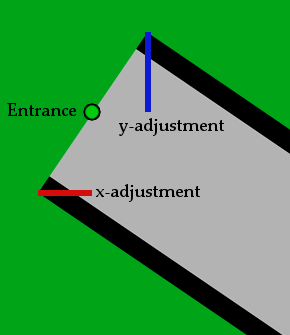
\includegraphics[height=7cm]{designNotes/adjustments.png}
\caption{A diagram indicating the x and y adjustments for the merging lane.}
\label{fig:adjustments}
\end{figure}

To get the Y-coordinate we can calculate the distance the coordinate is above the target lane, and then add the width of the target lane to that. We can also use this length to calculate the height of the whole simulator. However, to do that we will also need to add a y-adjustment, also shown in Figure \ref{fig:adjustments}.

Merge vehicles will exit the merge zone in the same place as target vehicles (equation \ref{targetLaneZoneExitX}), however, they will enter the merge zone at the top. The Y-coordinate of this point is equal to the width of the target lane. The X-coordinate is given by equation \ref{mergeLaneZoneEntranceX}.

\begin{equation}\label{mergeLaneZoneEntranceX}
	\begin{split}
mergeLaneZoneEntranceX = & width \\
						 & - targetLeadOutDistance \\
						 & - \frac{mergeZoneWidth}{2}
	\end{split}
\end{equation}

After the merge vehicles enter the merge zone they will deviate from the lane, however the lane itself continues until it reaches the centre of the target lane. We know this centre has a Y-coordinate equal to half of the lane width. The X-coordinate is more difficult to calculate. We need to find another X-adjustment, denoted as centreXAdjustment, along the target lane centre line. We can then use equation \ref{connectionPointX} to find the X-coordinate. Figure \ref{fig:centreXAdjustment} indicates the position of centreXAdjustment.

\begin{equation}\label{connectionPointX}
	\begin{split}
connectionPointX = & width \\
				   & - targetLeadOutDistance \\
				   & - \frac{mergeZoneWidth}{2} \\
				   & + centreXAdjustment \\
	\end{split}
\end{equation}

\begin{figure}[htb]
\centering
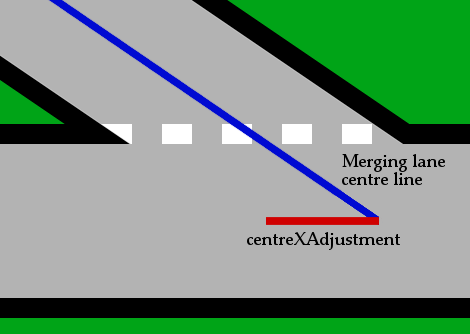
\includegraphics[height=8cm]{designNotes/centreXAdjustment.png}
\caption{A diagram indicating the X-adjustment used to find the point at which the two lanes connect.}
\label{fig:centreXAdjustment}
\end{figure}.

\section{Autonomous Merge Management System}
\label{sec:Autonomous Merge Management System}
This centralised system is based on the AIM system \citep{Dresner2004}. Once in range, approaching vehicles send a request message to the system with their vehicle specification and their predicted arrival time and arrival velocity. A vehicle specification contains a vehicle's maximum velocity, length, width, maximum acceleration and maximum deceleration.

Upon receiving a request the management system simulates the vehicle's journey through the merge zone, which has been split into a grid. As the vehicle is simulated, the system system notes the cells the vehicle moves through and the times at which it occupies each cell. The system then compares these 'space-time' values to its reservation store. The reservation store consists of sets of space-time values indicating where and when vehicles are expected to be in the merge zone. If the requesting vehicle does not clash with any of these reservations then the request is granted and the reservation store is updated. If not, the system rejects the request. The requesting vehicle will have to try and make a new reservation. They cannot enter the merge zone until they obtain a reservation.

Vehicles with a reservation continue towards the merge zone at the speed which allows them to enter at their scheduled arrival time. If a vehicle cannot maintain their reservation for any reason, it is their responsibility to alert the management system, at which point their reserved space-time values will be released and the vehicle will have to make a new reservation. Once a vehicle has successfully traversed the merge zone they will need to send a message to the management system to alert the system that they are leaving its zone of control. 

This system makes good use of space-time, allowing multiple vehicles into the merge zone at the same time. However, the system does have a number of issues. The primary one is that the leading vehicles in both lanes, that is the ones before the merge zone, will always be the only two with reservations. Lead vehicles are the only vehicles that can accurately predict their arrival time, as they don't have to consider the braking behaviour of any predecessors. A consequence of this is that successor vehicles very close behind the lead vehicle are forced to make a reservation very close to the merge zone. These vehicles have to slow in order to not enter the merge without a reservation, and as such experience reduced traffic flow.

Another problem is that the system does not guarantee that one lane will not experience large delays at the expense of another. If a vehicle on the target lane arrives first and makes a reservation, then a vehicle on the merge lane arrives and has to wait, there is nothing to say that twenty more target lane vehicles will pass through before the merge vehicle ever manages to make a reservation. A queued merge management system might be able to counteract this, as seen in section \ref{sec:Queue Merge Management System}.

\section{Queue Merge Management System}
\label{sec:Queue Merge Management System}
The queue merge management system is another approach to centralised vehicle control. In a reservation based system, where vehicles enter the merge at a pre-arranged time, a queued merge management system controls vehicles with a simple go/no-go system. Vehicles are sent messages telling them to enter the merge zone, without knowing exactly when that might be.

As a vehicle approaches the merge it sends a request to the management system. This request contains the vehicle's ID, the ID of the the vehicle's predecessor and the vehicle's distance to the merge zone. The predecessor ID and distance measurements are assumed to be accurate. In a real world scenario a vehicle could lie about these parameters, but as these parameters could be verified or collected by the management system instead, we assume them to be accurate.

An approaching vehicle has to be within a set distance of the merge zone in order to be added to the queue of vehicles being processed through the merge. This is mitigate the effect of very fast vehicles being forced to slow down, in order to allow slower vehicles earlier in the queue to pass through the merge zone. Any request from a vehicle further away from the merge zone that this distance is rejected.

If the vehicle's request is from within an acceptable distance, then the queue system checks to see if the vehicle's predecessor has been added to the queue. There is a possibility that the predecessor has not managed to make a request yet. This check ensures that the vehicle predecessor is added to the queue in a position before the vehicle. If the vehicle's predecessor has not yet been added the vehicle's request is rejected. Otherwise the vehicle's request is accepted with a confirmation message, and the vehicle's ID is added to the queue.

The vehicle is now awaiting a go message from the queue system. During this time it cannot enter the merge zone and must stop before it enters. The queue system sends go messages to vehicles in the queue as the previous vehicle that was sent a go message leaves the merge zone. This ensures that only one vehicle is in the merge zone at any time. Once a vehicle receives the go signal it must make its way towards the merge zone and traverse it. Once the vehicle leaves the merge zone it sends a message to the queue system confirming that it has safely traversed the merge and that it can let the next vehicle through.

This system sacrifices space efficiency for simplicity and a focus on fair access across both lanes. The system cannot have more than two vehicles in the merge zone at the same time, as the AIM-based system can. However, multiple vehicles on the same lane can be placed into the queue at any time, and the queue system does consider each lane equally, with no preference given to any one lane.

\section{Decentralised Merge Management System}
\label{sec:Decentralised Merge Management System}
The decentralised merge management system is based heavily on the work by VanMiddlesworth et al. in \citetitle{VanMiddlesworth2008} \citep{VanMiddlesworth2008}. This system is based on two message types, which each vehicle broadcasts to every other vehicle within range. The first message type is a \emph{Claim}. This message is used to try and reserve access to the merge zone. It contains the vehicle's ID, lane, estimated arrival time, estimated exit time and a boolean indicating whether or not it has stopped at the merge. The second message type is a \emph{Cancel}, used to release any reservations held by a vehicle. \emph{Cancel} messages contain a vehicle's id. All message types also contain a message ID which monotonically increments with each new message sent by the vehicle. Vehicles broadcast both message types repeatedly with a constant period to ensure that the messages are received by all other vehicles. 

Again we assume all of the values provided by the vehicles are accurate. VanMiddlesworth \citep{VanMiddlesworth2008} goes into further detail over dealing with selfish and malicious agents, however in this scenario we are assuming all vehicles are forced to provide accurate information.

Claims can compete with each other, in which case Claim dominance must be established. A claim $C_1$ dominates another claim $C_2$ if its $C_1$'s vehicle is stopped at the merge and $C_2$'s vehicle is not. Or if $C_1$ and $C_2$ are either both stopped at the merge or both not stopped at the merge, and $C_1$ has priority over $C_2$. Priority is indicated by the following rules, in order of evaluation:

\begin{enumerate}
\item \emph{If neither vehicle is stopped at the merge} The \emph{Claim} with the earliest exit time has priority.
\item \emph{If both vehicles are stopped at the merge} The \emph{Claim} on the target lane has priority. This is because in real world scenarios target lanes generally move more quickly than merge lanes.
\item \emph{Otherwise...} The vehicle with the lowest ID has priority
\end{enumerate}

As a vehicle approaches the merge it will receive messages from other agents. Before acting the vehicle 'lurks', long enough to be reasonably sure of every pending \emph{Claim} message. The vehicle then generates it's own \emph{Claim} message based on the earliest possible arrival and exit time of the vehicle. Once a vehicle has a \emph{Claim} they will continue broadcasting until they either complete the merge or have to change it. Once in the merge, the vehicle traverses in the manner their \emph{Claim} indicates. They continue broadcasting their \emph{Claim} during this time, but it cannot be dominated. 

If the vehicle's arrival estimation changes (due to predecessor vehicle braking or something similar) the vehicle generates a new \emph{Claim}. If another vehicle arrives at the merge before they do, the vehicle broadcasts \emph{Cancel} repeatedly with the same period as \emph{Claim}. This helps to deal with the lead vehicle only problem found in section \ref{sec:Autonomous Merge Management System}. Once cancelled the vehicle then attempts to make a new \emph{Claim}.

This system has the advantage of being completely decentralised, requiring no extra infrastructure to handle requests. However, the complexity of this system is far higher, requiring multiple agents to perform complex simulations and attempt to maintain a global picture of the system. In a centralised system, these activities are far easier to organise.